\documentclass[acmsmall,screen]{acmart}

%% acmart already loads amsmath (via amsart) and amssymb-equivalent symbols
%% (via newtxmath); loading amssymb again here conflicts with newtxmath's
%% \Bbbk definition, so it is deliberately omitted.
\usepackage{tikz}
\usetikzlibrary{positioning,arrows.meta}

%% ACM Transactions on Knowledge Discovery from Data (TKDD) metadata.
%% acmJournal/acmDOI/acmArticle etc. are placeholders until acceptance --
%% the venue's production team assigns real values at that point.
\acmJournal{TKDD}
\copyrightyear{2026}
\acmYear{2026}
\setcopyright{acmlicensed}
\acmDOI{XXXXXXX.XXXXXXX}

\title{When Imbalance Correction Backfires: Machine Learning Robustness of Tabular
Imbalance Mitigation Under Minority-Label Contamination}

\author{Sanjeev K. Khatri}
\email{sanjeev.khatri@trojans.dsu.edu}
\affiliation{%
  \institution{The Beacom College of Computer and Cyber Sciences, Dakota State University}
  \city{Madison}
  \state{SD}
  \country{USA}
}

\author{Zainab Albujasim}
\email{Zainab.Albujasim@dsu.edu}
\affiliation{%
  \institution{The Beacom College of Computer and Cyber Sciences, Dakota State University}
  \city{Madison}
  \state{SD}
  \country{USA}
}

\author{Youssef Harrath}
\email{youssef.harrath@dsu.edu}
\affiliation{%
  \institution{The Beacom College of Computer and Cyber Sciences, Dakota State University}
  \city{Madison}
  \state{SD}
  \country{USA}
}

\renewcommand{\shortauthors}{Khatri et al.}

%% CCS concepts: placeholders generated from the standard 2012 ACM CCS tree.
%% Verify/regenerate via https://dl.acm.org/ccs before final submission.
\begin{CCSXML}
<ccs2012>
<concept>
<concept_id>10010147.10010257.10010293.10010294</concept_id>
<concept_desc>Computing methodologies~Supervised learning by classification</concept_desc>
<concept_significance>500</concept_significance>
</concept>
<concept>
<concept_id>10010147.10010257</concept_id>
<concept_desc>Computing methodologies~Machine learning</concept_desc>
<concept_significance>300</concept_significance>
</concept>
</ccs2012>
\end{CCSXML}

\ccsdesc[500]{Computing methodologies~Supervised learning by classification}
\ccsdesc[300]{Computing methodologies~Machine learning}

\keywords{class imbalance, label noise, imbalance correction, TabPFN, XGBoost, calibration}

\begin{document}

\begin{abstract}
Under severe class imbalance, a classifier can achieve high overall accuracy
while performing poorly on the minority class that imbalance-correction
methods are intended to protect. Methods such as resampling, cost-sensitive
reweighting, and TabPFN posterior rescaling are typically evaluated under the
assumption of reliable labels, yet they may be deployed in settings where
labels are imperfect. Considerably less is known about whether these methods
remain beneficial when minority labels are corrupted. This paper addresses
that gap through a controlled audit of seven correction methods across TabPFN
(threshold correction, DistPFN, DistPFN-T, and downsampling) and XGBoost
(cost-sensitive weighting, random oversampling, and SMOTE). Two directed
label-noise mechanisms, majority-to-minority mislabeling and minority loss,
are injected across 26 UCI datasets, four imbalance ratios, five contamination
levels, and 10 seeds. Five metrics proposed in this paper assess correction
performance, while dataset-level Friedman and pairwise Wilcoxon tests assess
statistical significance. Across 112{,}319 evaluations, every correction
underperformed its baseline under some conditions, with harm rates ranging
from 2.4\% to 47.4\%. Excluding the balanced control lowers the maximum harm
rate to 37.8\%. Some corrections became non-beneficial at contamination levels
as low as 5\%, and method differences were significant in both model families
and both noise directions ($p < 10^{-9}$). TabPFN threshold correction was the
most robust, with the lowest harm rate and the highest mean gain in both
directions. Providing TabPFN's rescaling procedure with the true prior did not
consistently improve performance, suggesting that mislabeled context examples
may drive degradation. Resampling methods duplicate mislabeled examples, while
cost-sensitive and rescaling methods inherit the corrupted class ratio.
Scientifically, the study contributes a design that holds training size fixed,
preventing class ratio from being confounded with data volume. Practically,
the findings suggest that imbalance corrections should be evaluated under
realistic label noise before deployment.

\end{abstract}

\maketitle

\section{Introduction}
\label{sec:introduction}

In supervised classification, a model learns to predict a label, or class, for
each example from its features. Many practical
classification tasks have unequal class distributions. Examples in this study
include credit default, bankruptcy, and failures of Scania trucks (APS Failure),
where the rare outcome is the one the system is intended to detect. Misclassifying
a rare outcome can cost more than misclassifying a common one
\cite{elkan2001costsensitive}, which is why recognizing the minority class
matters. This situation is known as class imbalance: one class is substantially less frequent
than the other, which can degrade the model's ability to recognize the minority
class. Under severe skew, a classifier may achieve deceptively high overall
accuracy while exhibiting poor minority-class recall, because correct
predictions on the majority class can dominate the aggregate evaluation metric.

To address this, practitioners commonly turn to three kinds of correction.
Data-level resampling techniques, such as SMOTE~\cite{chawla2002smote} and random
oversampling, add or duplicate minority examples before training begins.
Cost-sensitive reweighting~\cite{elkan2001costsensitive} instead leaves the data
untouched and penalizes mistakes on the minority class more heavily during
training. A third kind, threshold and posterior-probability correction such as
DistPFN~\cite{lee2026distpfn}, is suited to tabular foundation models such as
TabPFN~\cite{hollmann2023tabpfn,hollmann2025tabpfnv2}. Instead of touching the data
or the training process, it adjusts the model's predictions after they have
already been made.

Many imbalance-correction strategies are evaluated under an implicit condition:
that the labels used to identify and characterize the minority class are
sufficiently reliable. Although class imbalance and label noise have each been
studied extensively, considerably less is known about whether standard imbalance
corrections remain beneficial when minority-label information is systematically
corrupted (Section~\ref{sec:related-work}).

If that assumption does not hold, none of these corrections can tell a genuine
minority example from a mislabeled one. A resampling method will duplicate or
synthesize around a mislabeled row exactly as readily as a correctly labeled one. A
cost-sensitive method will derive its penalty from the observed class ratio, so any
corruption in that ratio carries directly into the penalty. A posterior-rescaling
method will correct a prediction against an observed class prior that carries the
same corruption. In every case, the correction can end up amplifying the
mislabeled examples it was built to compensate for, rather than correcting for
genuine class imbalance.

This paper tests that failure mode directly, measuring when standard
imbalance-correction methods help and when they backfire under controlled, directed
label contamination. We organize this investigation around four research
questions.

\begin{itemize}
\item \textbf{RQ1.} Do standard imbalance corrections remain beneficial once
directed label error is present?
\item \textbf{RQ2.} How do correction failure rates differ between the two
directed corruption mechanisms?
\item \textbf{RQ3.} At what contamination rate does each correction stop paying off?
\item \textbf{RQ4.} How much of a correction's failure comes from using a
corrupted prior instead of the true, oracle prior?
\end{itemize}

Concretely, we audit seven correction methods across two widely deployed tabular
model families, TabPFN and XGBoost~\cite{chen2016xgboost}, under two directed,
asymmetric label-error mechanisms and a range of imbalance levels, using 26 real
datasets drawn from the UCI Machine Learning Repository~\cite{kelly_uci}. The design
holds the total amount of training evidence fixed across imbalance levels, so that
changes in imbalance are not confounded by changes in how much training evidence a
method receives. Section~\ref{sec:methods} gives the full experimental setup, including
the exact corruption procedure and every configuration tested.

To answer these questions, we judge whether a correction helps or hurts, rather
than only how accurate it is, using five purpose-built metrics. Correction Gain and
Correction Harm Rate answer RQ1 and RQ2, measuring whether and how often a
correction underperforms its uncorrected baseline. The break-even contamination
rate answers RQ3, and the Prior Sensitivity Gap answers RQ4. A fifth metric,
Regret, does not map onto a single research question. It measures how severe a
failure is when one occurs, complementing Correction Harm Rate's count of how
often one does. Each metric is defined precisely in Section~\ref{sec:methods}.

Our central finding is that every correction method tested underperforms its
matched uncorrected baseline in at least some conditions. How often this happens
depends strongly on both the direction of the corruption and the dataset the
correction is applied to, and no correction remains non-degrading across every
tested condition in both corruption directions. The complete results, including
per-method failure rates and break-even points, are reported in
Section~\ref{sec:results}.

Our contributions are as follows.

\begin{itemize}
\item We introduce a controlled experimental design that holds total training-set
size fixed across imbalance ratios, so that changes in training-set size are not
confounded with changes in class imbalance, and injects two directed, asymmetric
label-error mechanisms at every tested ratio.
\item We audit seven correction methods across two widely used model families,
including DistPFN and DistPFN-T~\cite{lee2026distpfn}. We validate our DistPFN and
DistPFN-T implementation against the authors' published reference code and document
an implementation error identified during this verification process
(Section~\ref{sec:methods}).
\item We operationalize correction robustness using five complementary measures,
Correction Gain, Correction Harm Rate, Regret, break-even contamination rate,
and Prior Sensitivity Gap, designed to measure whether a correction remains
net-beneficial once label noise is present, rather than measuring model
accuracy alone.
\item We show, across 26 real datasets, that every correction method tested can
underperform doing nothing at all once contamination reaches as little as 5\%, and
that this failure is direction-dependent rather than uniform across methods or
datasets.
\end{itemize}


\section{Related Work}
\label{sec:related-work}

\subsection{Tabular Foundation Models and In-Context Learning}

TabPFN~\cite{hollmann2023tabpfn} introduced a transformer pretrained once on
millions of synthetic datasets that performs supervised tabular classification
through in-context learning, the training set is presented as a prompt, and a
single forward pass yields predictions for the entire test set, without any
gradient-based fitting on the target data. The follow-up TabPFN~v2
release~\cite{hollmann2025tabpfnv2} scaled the pretraining prior and
architecture, reporting accuracy that matches or exceeds tuned gradient-boosted
ensembles on datasets of up to ten thousand rows while running orders of
magnitude faster. A concurrent empirical comparison across classical,
deep-learning, and tabular foundation models on imbalanced clinical
data~\cite{brima2026robustness} found that TabPFN~v2 and a related
in-context model, TabICL, rank competitively with tuned gradient-boosted
ensembles on one imbalanced clinical dataset but fall to intermediate,
less stable ranks on another, with XGBoost the only model family stable
across both. That comparison, like the TabPFN~v2 release itself, evaluates
imbalance robustness only under clean, uncorrupted labels, leaving open
whether either family's apparent robustness to imbalance survives once
label quality is also compromised, the question this paper asks directly.
Because a Prior-Data Fitted Network's predictions are shaped
entirely by the class distribution implicit in its pretraining prior together
with the context it is given, its behavior under a training-time class
distribution that differs from what the prior assumes is a distinct concern
from that of a conventionally trained classifier, and has only recently begun
to receive dedicated attention. Hu and Ghelichi~\cite{hu2026noiseimmunity}
take a complementary approach, analyzing TabPFN's internal attention
mechanisms directly under synthetic label-quality degradation and finding
that its attention stays structured and its ROC-AUC stays high without any
correction applied at all. Their analysis targets the model's internals
rather than the correction methods practitioners actually deploy on top of
it, the gap this paper's audit addresses.

DistPFN~\cite{lee2026distpfn} is the newest instance of a much older idea,
adjusting a classifier's output probabilities to match a known or assumed
target class prior, without retraining, first formalized for conventional
probabilistic classifiers by Saerens et al.~\cite{saerens2002adjusting}. To
our knowledge, DistPFN is the first method to bring this idea to an
in-context tabular foundation model, where the ``prior'' being adjusted for
is implicit in the pretrained transformer rather than an explicit model
parameter: it rescales TabPFN's predicted class probabilities to counteract
label shift between the training context and the deployment distribution,
with a temperature-scaled variant (DistPFN-T) that adapts the adjustment
strength to the discrepancy between the observed and reference priors. Both
variants require no retraining or architectural change, which places them in
the same class-imbalance setting that classical resampling and
cost-sensitive techniques were designed for on conventional classifiers,
despite operating through a completely different mechanism.

\subsection{Correcting Class Imbalance}

The dominant strategies for class imbalance fall into three families:
data-level resampling, algorithm-level cost adjustment, and, for
in-context tabular models, the test-time posterior corrections described
above. SMOTE~\cite{chawla2002smote} synthesizes new minority-class examples by
interpolating between real minority points and their nearest minority
neighbors in feature space, rather than duplicating existing rows, and remains
one of the most widely adopted correction techniques nearly a quarter-century
after its introduction. Random oversampling, by contrast, corrects the
training distribution by duplicating existing minority rows without
synthesizing new feature vectors. Both are implemented as standard,
interchangeable components in imbalanced-learn~\cite{lemaitre2017imbalancedlearn},
a widely used toolbox implementing both corrections. Cost-sensitive
learning~\cite{elkan2001costsensitive} instead leaves the training
distribution untouched and reweights the loss so that minority-class errors
are penalized more heavily than majority-class errors in proportion to the
observed class ratio. XGBoost's \texttt{scale\_pos\_weight}
parameter~\cite{chen2016xgboost} is a direct, widely used implementation of
this idea. Whether these
corrections reliably help at all, even when every label is trustworthy, is
itself contested: Elor and Averbuch-Elor~\cite{elor2022smote} find that with
a sufficiently strong classifier and well-chosen hyperparameters, balancing
the training set often provides no benefit over the imbalanced data as-is,
and can be actively counterproductive, a finding that already complicates
the assumption that these corrections are safe by default, before label
noise is introduced at all. All of these methods share a further, implicit
assumption that is central to this paper, that the
observed class labels used to compute the resampling ratio, the interpolation
neighborhood, or the cost ratio are themselves trustworthy. These classical corrections were not originally designed for robustness
to label noise. Subsequent empirical work, discussed later in this
section, has evaluated several sampling approaches under noisy-label
settings, but considerably less is known about the newer test-time
posterior corrections built for tabular foundation models.

\subsection{Learning Under Label Noise}

A separate literature studies classification when the observed labels
themselves are corrupted, independently of any class imbalance. Early
theoretical work formalized class-conditional label noise, in which the
probability that a true label is flipped depends only on its true class, and
established conditions under which consistent classifiers can still be
recovered~\cite{natarajan2013noisylabels}. Asymmetric label noise, where the
flip probabilities differ across classes or flip in only one direction, was
shown to require different identifiability and denoising strategies than the
symmetric case~\cite{scott2013asymmetricnoise}, indicating that the direction
and structure of label corruption, not only its rate, can materially change
how a classifier should be corrected. Frénay and
Verleysen~\cite{frenay2014labelnoise} survey sources and taxonomies of label
noise and its effects on classifier robustness prior to the deep learning era,
while Song et al.~\cite{song2022noisylabelssurvey} survey the substantially
larger body of work on training deep networks to be robust to noisy labels,
including loss correction, sample selection, and label correction approaches.
Both surveys treat label noise as a phenomenon to be corrected or tolerated
during training. Neither the surveys nor the methods they catalog examine how
label noise interacts with a class-imbalance correction applied
\emph{alongside} it, which is the specific interaction this paper studies,
not by proposing a new noise-robust training method, but by auditing whether
existing, widely deployed imbalance corrections remain net-beneficial once
that assumption is violated.

\subsection{The Understudied Intersection: Imbalance Correction Under Noisy Labels}

Empirically auditing whether imbalance corrections hold up under label
noise has important precedent. Van Hulse and
Khoshgoftaar~\cite{vanhulse2009knowledge} trained more than two million
classifiers across seven datasets, eleven learners, and seven sampling
techniques, including random oversampling and SMOTE, while varying the
location and level of class noise, showing that the class receiving the
noise materially affects how learning and sampling procedures behave and
establishing that imbalance mitigation can interact strongly with label
noise in classical learning settings. Our study addresses a
complementary setting, We control the total training-set size across
imbalance ratios so that changes in training-set size are not confounded
with changes in class imbalance, and we extend the analysis to tabular
foundation models and recently proposed test-time posterior corrections
such as DistPFN and DistPFN-T.

A smaller body of work has begun to treat class imbalance and label noise as
jointly occurring problems rather than independent ones. Koziarski et
al.~\cite{koziarski2020ccr} combine a resampling step with a label-cleaning step
specifically for multi-class imbalanced data known to contain label noise.
Chen et al.~\cite{chen2021rsmote} and Li et al.~\cite{li2024wrnd} take a
related but more direct approach, redesigning SMOTE itself so that its
neighborhood-based interpolation is weighted by local sample density and
downweights or filters out likely-noisy minority points, rather than pairing
an unmodified SMOTE with a separate cleaning stage. Khanal et
al.~\cite{khanal2024activelabel} combine active learning with
noisy-label training to handle both problems together in imbalanced medical
image classification. Liu et al.~\cite{liu2024imbalancednoisy} observe that
standard loss-based sample selection for noisy-label training is itself biased
against minority classes, since under-learned tail classes and noise-corrupted
classes are both associated with high training loss and are consequently
difficult to tell apart. They propose a class-balanced sample selection
procedure with confidence-based augmentation to correct this bias during
training. A recent line of work inverts the relationship between the two
problems entirely: Hu et al.~\cite{hu2025beneficialnoise} show that
\emph{deliberately} injecting an asymmetric label noise model, engineered
specifically to counteract a classifier's biased decision boundary, can
rebalance an imbalanced classifier without resampling at all. Their result
and ours are not in tension. They show that noise designed in advance to
help, with its direction and magnitude chosen to correct a known bias, can
substitute for a resampling or reweighting step; we show that the standard
resampling and reweighting steps already in deployment cannot tell that
engineered noise apart from the generic, uncontrolled label errors a real
dataset actually contains, and so extend the same corruption-tolerance
assumption to the corrections themselves rather than to the raw
classifier. Each of these lines of work proposes a new algorithm for the
training-time mechanism of handling noisy labels under imbalance. None of them
evaluates whether the standard \emph{imbalance corrections already in widespread use}
(SMOTE, random oversampling, cost-sensitive reweighting, or, for the newer
class of tabular foundation models, test-time posterior adjustment and
class-balanced downsampling) continue to help, are neutral, or actively harm
performance once a controlled fraction of the labels they operate on are
themselves wrong. What remains open, to our knowledge, is whether these
corrections, applied to tabular foundation models under a directed,
asymmetric label-error rate, still improve on doing nothing at all rather
than merely being neutral or harmful. Closing that gap is what this
paper's controlled, cross-method audit is designed to do.


\section{Methods}
\label{sec:methods}

This section describes the full experimental design: the datasets, the
construction that holds training-set size fixed across imbalance ratios, the
two directed label-error mechanisms, the seven correction methods audited, the
metrics used to score them, and the statistical tests used to compare them.

\subsection{Overview}
\label{sec:methods-overview}

Figure~\ref{fig:pipeline} summarizes the pipeline applied to every dataset. A
dataset is split once into a training pool and a held-out test set, which stays
fixed and clean for the rest of that seed's run. Only the training side is
resampled and corrupted, and each correction method is fit on that side and
scored against the same held-out test set. A controlled sample is drawn
from the training pool at a target minority ratio $r$ and a fixed total size
$N_{\text{common}}$ (Section~\ref{sec:methods-ncommon}). A directed label error
is then injected into that sample at a contamination rate $c$, in one of two
directions (Section~\ref{sec:methods-corruption}), or left clean at $c{=}0$.
Every correction method (Section~\ref{sec:methods-corrections}) is fit on the
resulting training set and scored against the same held-out test set, and the
scores are converted into the metrics described in
Sections~\ref{sec:methods-metrics} and~\ref{sec:methods-contribution}. This is
repeated for every combination of dataset, seed, imbalance ratio, contamination
rate, and direction, and for every correction method, producing one row per
method per condition.

\begin{figure*}[t]
\centering
\resizebox{\linewidth}{!}{%
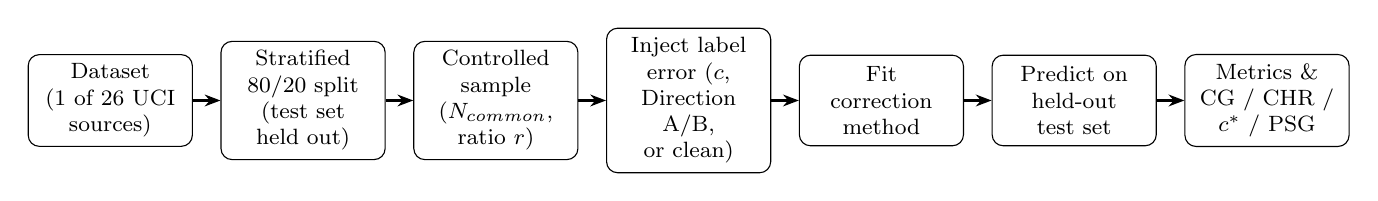
\begin{tikzpicture}[
  node distance=0.35cm,
  box/.style={draw, rounded corners, align=center, minimum height=1.15cm,
              text width=1.85cm, font=\footnotesize},
  arr/.style={-{Stealth[length=2mm]}, thick}
]
\node[box] (data) {Dataset\\(1 of 26 UCI\\sources)};
\node[box, right=of data] (split) {Stratified\\80/20 split\\(test set\\held out)};
\node[box, right=of split] (sample) {Controlled\\sample\\($N_{\text{common}}$,\\ratio $r$)};
\node[box, right=of sample] (corrupt) {Inject label\\error ($c$,\\Direction A/B,\\or clean)};
\node[box, right=of corrupt] (fit) {Fit\\correction\\method};
\node[box, right=of fit] (predict) {Predict on\\held-out\\test set};
\node[box, right=of predict] (score) {Metrics \&\\CG / CHR /\\$c^*$ / PSG};

\draw[arr] (data) -- (split);
\draw[arr] (split) -- (sample);
\draw[arr] (sample) -- (corrupt);
\draw[arr] (corrupt) -- (fit);
\draw[arr] (fit) -- (predict);
\draw[arr] (predict) -- (score);
\end{tikzpicture}%
}
\caption{Stress-cell pipeline, applied to each dataset, seed, ratio,
contamination rate, and direction.}
\label{fig:pipeline}
\end{figure*}

\subsection{Datasets}
\label{sec:methods-datasets}

Twenty-six binary-classification datasets were drawn from the UCI Machine
Learning Repository~\cite{kelly_uci}: Banknote
Authentication~\cite{lohweg2012banknote},
Blood Transfusion~\cite{yeh2008bloodtransfusion}, South German
Credit~\cite{groemping2019germancredit}, Spambase~\cite{hopkins1999spambase},
Breast Cancer Wisconsin~\cite{wolberg1993breastcancer},
Ionosphere~\cite{sigillito1989ionosphere}, Haberman's
Survival~\cite{haberman1999survival}, Statlog
Heart~\cite{statlogheart}, HTRU2~\cite{lyon2015htru2}, QSAR
Biodegradation~\cite{mansouri2013qsar}, Adult~\cite{becker1996adult},
Bank Marketing~\cite{moro2014bankmarketing}, MAGIC Gamma
Telescope~\cite{bock2004magic}, Online Shoppers Purchasing
Intention~\cite{sakar2018onlineshoppers}, Congressional Voting
Records~\cite{uci1987congressionalvoting}, Chronic Kidney
Disease~\cite{rubini2015ckd}, Default of Credit Card
Clients~\cite{yeh2009creditcard}, Taiwanese Bankruptcy
Prediction~\cite{uci2020taiwanbankruptcy}, Polish Companies
Bankruptcy~\cite{tomczak2016polishbankruptcy}, Mushroom~\cite{uci1981mushroom},
Cervical Cancer (Risk Factors)~\cite{fernandes2017cervical},
SECOM~\cite{mccann2008secom}, Arrhythmia~\cite{guvenir1997arrhythmia},
Internet Advertisements~\cite{kushmerick1999internetads},
Seismic-Bumps~\cite{sikora2010seismic}, and APS Failure at Scania
Trucks~\cite{scania2016apsfailure}, chosen so that no single result could be
attributed to one dataset's idiosyncrasies, spanning finance, security,
healthcare, signal processing, astronomy, chemistry, industrial
manufacturing, retail behavior, and political science. Each dataset
designates one binary class as its positive, or target, class
(Table~\ref{tab:datasets}); in the controlled training sets built in
Section~\ref{sec:methods-ncommon}, this class's prevalence is fixed to
$r$, so it is the minority class at every ratio below $r{=}0.50$ and
exactly balanced at $r{=}0.50$, regardless of how common or rare it is
in the original, unmodified dataset. Together they range
from 270 to 60,000 raw rows and from 3 to 1{,}558 raw features, and their
natural positive-class prevalence ranges from $1.7\%$ (APS Failure) to
$62.5\%$ (Chronic Kidney Disease, the one dataset in this study where the
positive class is the natural majority). Table~\ref{tab:datasets}
summarizes all 26 datasets' size, the controlled training size
$N_{\text{common}}$ every stress cell actually draws from, and the meaning
of the positive class in each. The $N_{\text{common}}$ column is the
controlled training size (Section~\ref{sec:methods-ncommon}) that every stress
cell draws from, not the raw row count. It is computed at seed 13, and
seed-to-seed variation is at most a few rows from stratified-split rounding.
Feature counts marked $\to$100 are capped (Section~\ref{sec:methods-datasets}).

\begin{table*}[t]
\centering
\caption{Dataset characteristics for all 26 datasets.}
\label{tab:datasets}
\begin{tabular}{@{}lrrrl@{}}
\toprule
Dataset & Rows & Feat. & $N_{\text{common}}$ & Positive class \\
\midrule
Banknote Authentication      & 1{,}372 & 4  & 641   & Forged banknote \\
Blood Transfusion             & 748    & 4  & 284   & Blood donated in target period \\
South German Credit           & 1{,}000 & 20 & 480   & Bad credit risk \\
Spambase                      & 4{,}601 & 57 & 2{,}347 & Spam email \\
Breast Cancer Wisconsin       & 569    & 30 & 300   & Malignant diagnosis \\
Ionosphere                    & 351    & 34 & 189   & No ionospheric structure \\
Haberman's Survival           & 306    & 3  & 128   & Death within 5 years \\
Statlog Heart                 & 270    & 13 & 126   & Heart disease present \\
HTRU2                         & 17{,}898 & 8 & 2{,}622 & Pulsar candidate \\
QSAR Biodegradation           & 1{,}055 & 41 & 568   & Ready biodegradable \\
Adult                          & 48{,}842 & 14 & 18{,}698 & Income exceeds \$50K/year \\
Bank Marketing                 & 45{,}211 & 16 & 8{,}462  & Client subscribed to term deposit \\
MAGIC Gamma Telescope          & 19{,}020 & 10 & 10{,}385 & Hadron (background) event \\
Online Shoppers                & 12{,}330 & 17 & 3{,}052  & Session ended in completed purchase \\
Congressional Voting           & 435     & 16 & 225    & Republican representative \\
Chronic Kidney Disease         & 400     & 24 & 126    & Chronic kidney disease present \\
Default of Credit Card Clients & 30{,}000 & 23 & 10{,}618 & Default on payment next month \\
Taiwanese Bankruptcy           & 6{,}819  & 95 & 352    & Company went bankrupt \\
Polish Companies Bankruptcy    & 43{,}405 & 65 & 3{,}346  & Bankrupt within forecast period \\
Mushroom                       & 8{,}124  & 22 & 3{,}543  & Poisonous mushroom \\
Cervical Cancer (Risk Factors) & 858     & 32 & 88     & Biopsy-confirmed abnormality \\
SECOM                          & 1{,}567  & 590$\to$100 & 166 & Semiconductor test fail \\
Arrhythmia                     & 452     & 279$\to$100 & 206 & Cardiac arrhythmia present \\
Internet Advertisements        & 3{,}279  & 1{,}558$\to$100 & 734 & Image is an advertisement \\
Seismic-Bumps                  & 2{,}584  & 18 & 272    & Hazardous seismic state next shift \\
APS Failure at Scania Trucks   & 60{,}000 & 170$\to$100 & 1{,}600 & APS component failure \\
\bottomrule
\end{tabular}
\end{table*}

No transformation altered the semantics of any feature. Two categories of
transformation changed feature values or feature counts, neither altering
what a feature means. First, column renames, purely cosmetic, applied to
Spambase and QSAR Biodegradation: XGBoost's tree serialization format
rejects the characters \texttt{[}, \texttt{]}, and \texttt{<} in feature
names, so Spambase's \texttt{char\_freq\_[} (the frequency of the
\texttt{[} character in an email) was renamed to
\texttt{char\_freq\_bracket\_open}, and eight of QSAR Biodegradation's
molecular-descriptor columns (e.g., \texttt{F01[N-N]}) had their brackets
replaced with a hyphen (e.g., \texttt{F01\_N-N}), with the underlying values
unchanged in both cases. Second, a feature cap applied to the four datasets
with more than 100 raw features, SECOM (590), Arrhythmia (279), Internet
Advertisements (1{,}558), and APS Failure (170): each is capped to a
deterministic random subsample of 100 columns (fixed seed, sorted for a
stable, reviewable column order), so that no method's training cost scales
with raw feature count rather than with the imbalance and noise conditions
actually under test. The columns kept are fixed once per dataset and
identical across every seed, ratio, and contamination level tested on it.

The pipeline separately includes leakage-safe median imputation for numeric
columns and most-frequent-value imputation followed by one-hot encoding for
categorical columns, fit only on each stress condition's training rows.
Ten of the 26 datasets, Banknote Authentication, Blood Transfusion, South
German Credit, Spambase, Breast Cancer Wisconsin, Ionosphere, Haberman's
Survival, Statlog Heart, HTRU2, and QSAR Biodegradation, contain no missing
values and no non-numeric feature column (South German Credit's twenty
attributes and Statlog Heart's categorical clinical measures are
integer-coded and are treated as numeric throughout), so neither step
alters any value for those ten. Of the remaining sixteen, eleven contain at
least one column with missing values (Adult, Bank Marketing, Congressional
Voting, Chronic Kidney Disease, Polish Companies Bankruptcy, Mushroom,
Cervical Cancer, SECOM, Arrhythmia, Internet Advertisements, and APS
Failure) and seven contain genuinely categorical, non-numeric columns
(Adult, Bank Marketing, Online Shoppers, Congressional Voting, Chronic
Kidney Disease, Mushroom, and Seismic-Bumps), so both imputation steps and
the one-hot encoding step are genuinely exercised in this study, rather
than being present in the pipeline but never triggered.

Before any sampling or corruption, each dataset is split once with a
stratified 80/20 train/test split, so both partitions preserve the dataset's
original class ratio. The test partition is fixed for that seed and never
altered by any later step. Every correction method, at every imbalance ratio
and contamination level, is scored against exactly the same test rows.

That fixed test partition has a consequence worth naming directly. Because
it is never resampled, it keeps each dataset's natural positive-class
prevalence throughout, while Section~\ref{sec:methods-ncommon} deliberately reshapes
the training partition to $r$. Natural prevalence across the 26 datasets
ranges from $1.7\%$ (APS Failure) to $62.5\%$ (Chronic Kidney Disease).
Seven datasets sit at or below the two most severe tested ratios: APS
Failure ($1.7\%$) and Taiwanese Bankruptcy ($3.2\%$) fall below even
$r{=}0.05$; Polish Companies Bankruptcy ($4.8\%$) sits almost exactly on
it; and Cervical Cancer ($6.4\%$), Seismic-Bumps ($6.6\%$), SECOM
($6.6\%$), and HTRU2 ($9.2\%$) all sit close to $r{=}0.10$. So at
$r{=}0.05$ and $r{=}0.10$ especially, training and test are drawn from
different class priors for a substantial share of the datasets in this
study. The severe-imbalance conditions this study emphasizes are therefore
not imbalance in isolation. They combine
imbalance with a train/test prior shift, exactly the kind of mismatch
DistPFN and DistPFN-T are built to correct
(Section~\ref{sec:methods-corrections}), and the kind
\texttt{tabpfn\_threshold}'s own threshold adjustment addresses as well.
Section~\ref{sec:discussion-simplicity} returns to what this means for
interpreting why the simplest corrections in this study lead, and
Section~\ref{sec:threats-internal} states the resulting limitation on
treating imbalance and prior shift as separable.

\subsection{Controlled Imbalance: A Common Training Size}
\label{sec:methods-ncommon}

Each dataset is tested at four minority ratios, $r \in \{0.50, 0.20, 0.10,
0.05\}$, where $r$ is the fraction of training rows that belong to the
minority class. Comparing a model trained at a high ratio (e.g., $r{=}0.20$)
against one trained at a low ratio (e.g., $r{=}0.05$) is only informative
about imbalance itself if both training sets are the same total size.
Otherwise, a difference in performance could be explained by sample size
rather than by imbalance. To remove that confound, one shared training size
$N_{\text{common}}$ is computed for each dataset and seed and used at every
tested ratio. Only the split between minority and majority rows within that
fixed total changes as $r$ changes.

Let $n_{\min}$ and $n_{\max}$ denote the number of positive-class and
other-class rows available in the training pool for a given dataset and
seed (named for their role in the controlled sample below, not for which
is numerically larger in the raw pool; Chronic Kidney Disease's positive
class is the raw pool's natural majority, Section~\ref{sec:methods-datasets}).
At ratio $r$, a
total training size of $N$ requires $rN$ minority rows and $(1-r)N$ majority
rows, so the largest $N$ achievable at that ratio is bounded by whichever
class runs out first:
\begin{equation}
\text{feasible\_n}(r) = \min\!\left(\frac{n_{\min}}{r},\ \frac{n_{\max}}{1-r}\right).
\label{eq:feasible-n}
\end{equation}
$N_{\text{common}}$ is the largest size achievable at every tested ratio
simultaneously, i.e., the tightest of these four constraints, floored to a
whole number of rows:
\begin{equation}
N_{\text{common}} = \left\lfloor \min_{r \in \{0.50,0.20,0.10,0.05\}} \text{feasible\_n}(r) \right\rfloor.
\label{eq:ncommon}
\end{equation}
For a given $r$ and $N_{\text{common}}$, a controlled training set is drawn by
sampling $\text{round}(r \cdot N_{\text{common}})$ minority rows and the
remaining $N_{\text{common}}$ rows from the majority class, both without
replacement, then shuffling the combined set.

\subsection{Directed Label-Error Mechanisms}
\label{sec:methods-corruption}

Two label-error mechanisms are applied to the controlled training set built
in Section~\ref{sec:methods-ncommon}, each at contamination rate $c \in
\{0.05, 0.10, 0.20, 0.30\}$, plus a shared clean condition at $c{=}0$. Both
flip a controlled number of true labels within that set, but they differ in
which class is flipped and how $c$ is defined relative to the resulting
pool. Here $n_{\min}$ denotes the number of true minority rows in that
controlled training set, equal to $\text{round}(r \cdot N_{\text{common}})$
by construction, not the pool-level $n_{\min}$ from
Section~\ref{sec:methods-ncommon}.

\textbf{Direction A (contamination): majority rows relabeled as minority.}
$c$ is defined as the fraction of the \emph{observed} minority-labeled pool
that is actually mislabeled majority rows. If $k$ majority rows are
flipped,
\begin{equation}
c = \frac{k}{n_{\min} + k}
\quad\Longrightarrow\quad
k = \frac{c}{1-c}\, n_{\min}.
\label{eq:directionA}
\end{equation}
$k$ rows are drawn uniformly at random from the majority pool and relabeled.

\textbf{Direction B (loss): minority rows relabeled as majority.}
Here $c$ is defined directly against the true minority count:
\begin{equation}
k = c \cdot n_{\min}.
\label{eq:directionB}
\end{equation}
$k$ rows are drawn uniformly at random from the minority pool and relabeled.

Both mechanisms return the corrupted labels together with the realized
contamination rate (which can differ slightly from the requested $c$ due to
integer rounding of $k$) and the indices flipped, so every corruption is
fully auditable. This asymmetric, class-conditional construction follows the
label-noise formalization of Natarajan et al.~\cite{natarajan2013noisylabels}
and Scott et al.~\cite{scott2013asymmetricnoise}, rather than symmetric random
flipping.

That difference in definition is not cosmetic. Direction A's $c$ describes
contamination as it would be observed after the fact, the fraction of
everything now labeled minority that is actually a mislabeled majority row,
close to asking how many flagged cases turn out to be false alarms.
Direction B's $c$ instead measures signal loss directly against the true
minority count, the fraction of genuine minority rows destroyed. The two are
natural for the process each direction represents, but they are not the
same quantity. The same nominal $c$ therefore corresponds to a different
flip count relative to $n_{\min}$ in each direction. At $c{=}0.30$,
Direction A flips $k/n_{\min} = c/(1-c) = 42.9\%$ of $n_{\min}$'s worth of
majority rows, while Direction B flips exactly $30\%$, a gap that widens
with $c$ (from $5.3\%$ against $5.0\%$ at $c{=}0.05$) but stays independent
of $r$, since both ratios are taken relative to $n_{\min}$ within their own
direction's formula rather than against the majority count. Comparing
directions at matched nominal $c$, as Section~\ref{sec:results-rq2} does,
is therefore a comparison of each direction's own natural severity, not of
an identical absolute flip count, a distinction
Section~\ref{sec:threats-internal} returns to.

\subsection{Correction Methods}
\label{sec:methods-corrections}

Seven correction methods are audited, split into two families so that every
method is compared against the uncorrected baseline for the same underlying
model. All XGBoost variants share one frozen configuration
(Table~\ref{tab:config}), never tuned per condition, so any performance
difference between them is attributable to the correction technique itself.

\subsubsection{XGBoost family}

\texttt{xgb\_none} trains XGBoost~\cite{chen2016xgboost} directly on the
corrupted, imbalanced training set with no correction, and is the baseline
every other XGBoost variant is measured against. \texttt{xgb\_weighted} sets
\texttt{scale\_pos\_weight} to the ratio of observed majority to observed
minority rows, following the cost-sensitive framing of
Elkan~\cite{elkan2001costsensitive}. \texttt{xgb\_ros} applies random
oversampling, duplicating minority-labeled rows with replacement until the
classes are balanced. \texttt{xgb\_smote} instead synthesizes new
minority-labeled rows with SMOTE~\cite{chawla2002smote}, interpolating
between a minority row and one of its $k$ nearest minority neighbors, a
parameter unrelated to the flip count $k$ in
Section~\ref{sec:methods-corruption}. It is set to
$k = \min(5,\, n_{\min}^{\text{obs}}-1)$, where $n_{\min}^{\text{obs}}$ is the
observed minority count in the corrupted training set actually being
resampled (distinct from both $n_{\min}$ in
Section~\ref{sec:methods-ncommon} and $n_{\min}$ in
Section~\ref{sec:methods-corruption}), so the request never exceeds the
neighbors actually available. Both resampling variants use
imbalanced-learn~\cite{lemaitre2017imbalancedlearn}.

\subsubsection{TabPFN family}

TabPFN~\cite{hollmann2023tabpfn,hollmann2025tabpfnv2} is an in-context tabular
foundation model: it is not fit with gradient descent on the study's data, but
reads the entire training set as a prompt and produces a prediction for each
test row in a single forward pass. Every TabPFN variant uses the library's
default hyperparameters, with only the random seed set per run, so no
TabPFN-specific configuration table is needed alongside
Table~\ref{tab:config}. \texttt{tabpfn\_none} takes its raw
$P(\text{minority})$ and thresholds at 0.5, and is the baseline for the rest
of the family. \texttt{tabpfn\_threshold} instead thresholds at $\pi$, the
class-1 prior used for correction, following the classical
posterior-adjustment principle of Saerens et al.~\cite{saerens2002adjusting}:
predict minority if $P(\text{minority}) > \pi$. As with every prior-dependent
method in this family, $\pi$ is either the observed, possibly corrupted
training rate $\pi_{\text{obs}}$ (the deployable variant) or the true
pre-corruption rate $\pi_{\text{true}}$ (the oracle diagnostic described in
Section~\ref{sec:methods-contribution}).

\texttt{tabpfn\_distpfn} and \texttt{tabpfn\_distpfn\_t} implement
DistPFN and DistPFN-T~\cite{lee2026distpfn}. Writing $p$ for TabPFN's raw
2-class prediction on one test row and $\bar{p}$ for the mean of $p$ across
the whole test batch,
\begin{equation}
\text{prior} = [1-\pi,\ \pi], \qquad
\text{adjusted} = \text{Normalize}\!\left(\frac{p \cdot \bar{p}}{\text{prior}}\right),
\label{eq:distpfn}
\end{equation}
using the same class-1 prior $\pi$ (observed or oracle, as defined above).
DistPFN-T adds a shared temperature
$\tau$ before the same final step:
\begin{equation}
\tau = -\sum_i \bar{p}_i \log(\text{prior}_i), \qquad
\bar{p}_T = \text{softmax}(\bar{p}/\tau),
\label{eq:distpfnt}
\end{equation}
with $\bar{p}_T$ substituted for $\bar{p}$ in Equation~\ref{eq:distpfn}. Both
formulas were verified directly against the authors' official reference
implementation before use in this study. That verification surfaced a
defect in the reference implementation itself, reported here rather than
left implicit: the authors' own published DistPFN-T reference driver
raises a shape error (\texttt{numpy}'s \texttt{AxisError}) for binary
classification, which its own exception handling silently swallows, so the
reference driver as published cannot produce a DistPFN-T score for a
two-class problem. Equation~\ref{eq:distpfnt} implements the algorithm's
evident intent, with that shape bug corrected rather than reproduced.

\texttt{tabpfn\_downsample} is the family's one data-level correction:
whichever class has more observed rows is randomly downsampled, without
replacement, to match the observed count of the smaller class, and TabPFN
reads the resulting balanced set as its prompt. Identifying the larger
class from the observed labels directly, rather than assuming a fixed
encoding stays the larger one, means this never fails regardless of how
contamination shifts the observed class balance, including at $r{=}0.50$
under Direction A, where relabeling majority rows as minority can push
the observed minority count above the observed majority count.

For prior-dependent methods (\texttt{tabpfn\_threshold},
\texttt{tabpfn\_distpfn}, \texttt{tabpfn\_distpfn\_t}), every stress cell
(one dataset, seed, ratio, contamination rate, and direction) is scored
twice: once using the observed prior $\pi_{\text{obs}}$, the only
value available in a real deployment, and once using the oracle prior
$\pi_{\text{true}}$, the clean pre-corruption rate, which a real system could
never know. The oracle variant exists only to compute the Prior Sensitivity
Gap (Section~\ref{sec:methods-contribution}) and is never treated as a
deployable result.

\subsection{Evaluation Metrics}
\label{sec:methods-metrics}

Every method, on every stress cell, is scored with ten metrics computed
against the fixed, clean test set: balanced accuracy, worst-class recall
(the lower of the two per-class recalls, which catches a collapse in one
class that balanced accuracy alone can hide), area under the
precision-recall curve (AUPRC), macro-averaged F1, minority-class
precision and recall, area under the ROC curve (AUROC), Brier
score~\cite{brier1950verification}, log loss, and expected calibration
error (ECE, ten equal-width bins)~\cite{guo2017calibration}, which
measures how far a model's predicted probabilities are from the true
observed frequencies.

All ten are computed identically for every method and condition using
scikit-learn's implementations~\cite{pedregosa2011scikitlearn}, so no
method is scored on a different basis than any other.

Not every metric receives equal treatment in Section~\ref{sec:results}.
Balanced accuracy is reported as the discrimination measure throughout.
Worst-class recall, AUPRC, and macro F1 correlate with it at 0.968, 0.781,
and 0.919 respectively (Pearson, computed across the full result set) and
largely reproduce the same ranking rather than adding independent
evidence. AUPRC's correlation is the loosest of the three, consistent with
this study's wide range of natural imbalance producing real divergence
between the two metrics, but not loose enough to promote it from a
secondary diagnostic to a headline measure on its own. Minority precision,
minority recall, and AUROC are computed as
secondary diagnostics, available for a targeted check but not used to
support a headline claim on their own. Brier score and expected
calibration error are reported separately in
Section~\ref{sec:results-reliability} because together they reveal a
divergence from the discrimination results that balanced accuracy alone
does not show (Section~\ref{sec:discussion-calibration}). Log loss is
computed identically to the other nine metrics but is not separately
reported, since its correlation with Brier score, 0.959, is comparably
high and does not add evidence beyond it.

\subsection{Contribution Metrics}
\label{sec:methods-contribution}

The ten metrics above measure how good a method is in isolation. The
following five metrics are proposed in this paper. They are defined here for
this study, not taken from prior work, and they answer the question this study
is actually about: whether a correction is worth applying once label noise is
present, relative to doing nothing at all. All five compare a corrected method against its
matching uncorrected baseline (\texttt{xgb\_none} or \texttt{tabpfn\_none})
at the \emph{same} dataset, seed, ratio, contamination rate, and direction.

\textbf{Correction Gain (CG).} $S$ is first computed per seed, then
averaged across the ten seeds within each (dataset, $r$, $c$, direction)
block, for the corrected method and its uncorrected baseline separately.
CG is the difference of those two seed-averaged scores,
\begin{equation}
\text{CG} = \bar{S}_{\text{corrected}} - \bar{S}_{\text{uncorrected}},
\label{eq:cg}
\end{equation}
sign-adjusted so that positive always means the correction helped: unchanged
for metrics where higher is better (balanced accuracy, AUPRC), and negated
for loss-type metrics where lower is better (Brier score, log loss). CG,
and every metric built from it below, therefore has one value per (method,
dataset, $r$, $c$, direction) block, not one value per stress cell; a
single seed's evaluation never counts as a unit of evidence on its own.
For the one block affected by the failure disclosed in
Section~\ref{sec:methods-implementation} (\texttt{tabpfn\_downsample} on
APS Failure, $r{=}0.10$, $c{=}0.05$, Direction A), $\bar{S}_{\text{corrected}}$
averages the nine seeds that completed rather than ten, while
$\bar{S}_{\text{uncorrected}}$ for that same block still averages all ten,
since the failure was specific to the corrected method's fit, not the
baseline's; this affects one of 416 blocks for that method and direction.

\textbf{Correction Harm Rate (CHR).} Across every (dataset, $r$, $c$,
direction) block tested for one method,
\begin{equation}
\text{CHR} = \frac{\#\{\text{blocks with CG} < 0\}}{\#\{\text{blocks tested}\}}.
\label{eq:chr}
\end{equation}
With 26 datasets, four ratios, and four nonzero contamination rates, this
is 416 blocks per method and direction (Table~\ref{tab:robustness}), not
the 4,160 individual seed-level evaluations a per-seed count would give.
CHR counts any negative seed-averaged gain as harmful, including
differences too small to distinguish from measurement noise.
Section~\ref{sec:results-rq1} also
reports a stricter variant that only counts a block as harmful once CG
falls below $-0.01$ on balanced accuracy, a sensitivity check on how much
of the headline rate reflects negligible differences rather than a
meaningful failure.

\textbf{Regret.} How large the harm is when a correction does fail, zero
otherwise:
\begin{equation}
\text{Regret} = \max(0,\ -\text{CG}).
\label{eq:regret}
\end{equation}
CHR answers how often a correction backfires. Regret answers how bad it is
when it does, so a method with low CHR but large Regret on the blocks where it
fails carries a different practical risk than one with high CHR but small
Regret.

\textbf{Break-even contamination rate ($c^*$).} For a method, dataset, and
imbalance ratio, $c^*$ is the smallest tested $c > 0$ at which the
seed-averaged CG first drops to zero or below. This marks the first noise
level a correction stops paying off, not necessarily the last, since CG is
not guaranteed to stay negative at every higher $c$ afterward
(Section~\ref{sec:threats-construct} quantifies how often it does not). If
CG never crosses zero within the tested range, $c^*$ is reported as greater
than the largest tested $c$ (0.30) rather than extrapolated beyond what was
actually measured.

\textbf{Prior Sensitivity Gap (PSG).} For the three prior-dependent TabPFN
methods,
\begin{equation}
\text{PSG} = S_{\text{oracle prior}} - S_{\text{observed prior}},
\label{eq:psg}
\end{equation}
comparing the real, deployable variant against the oracle diagnostic
described in Section~\ref{sec:methods-corrections}. A large positive PSG
means most of a correction's failure traces specifically to the prior being
wrong. A small PSG despite otherwise poor performance means the failure comes
from elsewhere.

As a robustness check on whether pooling the balanced condition
$r{=}0.50$ together with the three genuinely imbalanced ratios biases
these headline contribution metrics, Section~\ref{sec:results-r050}
recomputes CHR, mean CG, break-even share, PSG, and every statistical
test in Section~\ref{sec:methods-statistics} three times: once on the
full pooled set (as everywhere else in this paper), once restricted to
$r \in \{0.20, 0.10, 0.05\}$, and once restricted to $r{=}0.50$ alone.
All three use the identical formulas defined above, applied to the same
already-collected evaluations; no additional model fitting or scoring
was performed.

\subsection{Statistical Testing}
\label{sec:methods-statistics}

For each model family (XGBoost, TabPFN) and each corruption direction, the
methods in that family are compared using the Friedman
test~\cite{friedman1937ranks}, a non-parametric omnibus test for differences
among more than two related samples, applied to seed-averaged balanced
accuracy across every (dataset, $r$, $c$) block with a complete row for every
method in that family. For the three prior-dependent TabPFN methods, only
the observed-prior variant, the same deployable score reported everywhere
else in this study, enters the comparison. The oracle-prior rows are
excluded so that a method's column reflects its deployable score alone, not
an average of its observed and oracle variants. A family/direction
combination is tested only when at least ten complete blocks are
available; every combination in this study clears that bar by a wide
margin (416 condition-level blocks, 26 dataset-level blocks, per
family and direction), so the rule never excludes a comparison here but
is stated for reproducibility on a different data cut. When
the Friedman test is
significant at $p<0.05$, every pairwise comparison of methods within that
family and direction is tested with the Wilcoxon signed-rank
test~\cite{wilcoxon1945ranking}, and the resulting $p$-values are corrected
for multiple comparisons with Holm's step-down
procedure~\cite{holm1979sequential}.

Blocking by (dataset, $r$, $c$) treats every tested ratio and noise level
within one dataset as an independent unit of evidence, but conditions
drawn from the same dataset share its underlying feature distribution and
test set, so they are not fully independent of each other. As a more
conservative check, the same comparison is repeated with each dataset as
a single block ($n{=}26$), first averaging balanced accuracy within a
family and direction across every tested $r$ and $c$ for that dataset,
then applying the Friedman test to those 26 dataset-level values per
method, the standard practice for comparing algorithms across multiple
datasets~\cite{demsar2006statistical}. Every pairwise Wilcoxon comparison
is repeated at this same dataset-level block, Holm-corrected separately
from the (dataset, $r$, $c$) version, since a significant omnibus result
does not by itself establish that every individual pairwise difference
holds under the stricter standard. Section~\ref{sec:results-significance}
reports all versions.

\subsection{Implementation and Reproducibility}
\label{sec:methods-implementation}

Every (dataset, ratio, contamination rate, direction) combination is
repeated across all ten seeds (13, 37, 73, 5, 11, 17, 19, 23, 29, and 31),
producing one stress cell per seed, so no result depends on one particular
random split or one particular set of flipped rows. A
method failing on a given stress cell is
logged with its error rather than silently skipped, and does not stop any
other method or any later cell: one such failure occurred in the final run,
\texttt{tabpfn\_downsample} on APS Failure (seed 19, $r{=}0.10$,
$c{=}0.05$, Direction A) raised a singular-value decomposition
non-convergence error on that specific resampled training set, reproducibly
across repeated attempts, and is reported as a failure rather than
interpolated or dropped (Section~\ref{sec:results}). All other
$112{,}319$ of the $112{,}320$ planned evaluations completed.
Table~\ref{tab:config} records the exact software
versions, platform, and the frozen XGBoost configuration used throughout.
The TabPFN checkpoint used was \texttt{tabpfn-v3-classifier-v3\_default.ckpt}
(SHA-256~\texttt{d0d865d5\ldots8f3988}), and TabPFN inference used Apple's
Metal (MPS) GPU backend rather than CPU. Every library's internal thread
pool (OpenMP, BLAS) was forced to a single thread throughout the study,
because XGBoost and PyTorch, which TabPFN depends on, each bundle their own
threading runtime, and running both in the same process without this
restriction reproducibly hangs (or, in the reverse import order, segfaults).
At the dataset sizes used in this study, the resulting single-threaded
slowdown is negligible.

\begin{table}[t]
\centering
\caption{Software environment and frozen XGBoost configuration.}
\label{tab:config}
\begin{tabular}{@{}ll@{}}
\toprule
Component & Value \\
\midrule
\multicolumn{2}{@{}l}{\textit{Software versions}} \\
Python & 3.13.5 \\
Platform & macOS 26.5.1 (arm64) \\
NumPy & 2.5.2 \\
pandas & 3.0.5 \\
scikit-learn & 1.9.0 \\
SciPy & 1.18.0 \\
XGBoost & 3.4.1 \\
imbalanced-learn & 0.14.2 \\
statsmodels & 0.14.6 \\
TabPFN & 8.3.0 \\
Seeds & 13, 37, 73, 5, 11, 17, 19, 23, 29, 31 \\
\midrule
\multicolumn{2}{@{}l}{\textit{XGBoost configuration (frozen, all variants)}} \\
\texttt{n\_estimators} & 500 \\
\texttt{max\_depth} & 6 \\
\texttt{learning\_rate} & 0.05 \\
\texttt{subsample} & 0.8 \\
\texttt{colsample\_bytree} & 0.8 \\
\texttt{eval\_metric} & logloss \\
\bottomrule
\end{tabular}
\end{table}


\section{Results and Discussion}
\label{sec:results}

The 26 datasets, ten seeds, four imbalance ratios, and five contamination
conditions (the shared clean condition plus four noise levels in each of the two
directions) form 9{,}360 stress cells. Nine methods (seven corrections plus the
two uncorrected baselines) are scored on every cell, giving 84{,}240 evaluations.
The three prior-dependent TabPFN corrections are also scored with the oracle
prior for diagnosis, adding 28{,}080 more. Of the 112{,}320 planned evaluations,
112{,}319 completed. The exception is \texttt{tabpfn\_downsample} on APS Failure
(seed 19, $r{=}0.10$, $c{=}0.05$, Direction A), which failed to converge
(Section~\ref{sec:methods-implementation}) and is excluded from the tables rather
than interpolated.

\subsection{Overall Correction Robustness}
\label{sec:results-rq1}

Every one of the seven correction methods produced at least one (dataset, $r$,
$c$, direction) block with negative Correction Gain, so no correction is
uniformly beneficial once label error is present. How often this happens varies
sharply by method. Table~\ref{tab:robustness} reports Correction Harm Rate (CHR)
and mean Correction Gain (CG, on balanced accuracy). \texttt{tabpfn\_threshold}
is the most robust method by both measures in both directions. Its CHR is 4.8\%
under Direction A and 2.4\% under Direction B, less than half the next-lowest
correction in either direction, and its mean CG (0.072 and 0.093) is the highest
of any method. The worst end of the table is the same in both directions.
\texttt{tabpfn\_distpfn} and \texttt{tabpfn\_distpfn\_t} have the highest CHR
under Direction A (35.1\% and 33.9\%) and, by a wider margin, under Direction B
(43.8\% and 47.4\%, more than five times the next-highest method there).

\begin{table}[t]
\centering
\caption{Correction Harm Rate and mean Correction Gain (balanced accuracy) over
noisy blocks ($c>0$), each averaged across ten seeds and pooled across datasets
and ratios ($n{=}416$ per method and direction).}
\label{tab:robustness}
\begin{tabular}{@{}lrrrr@{}}
\toprule
& \multicolumn{2}{c}{CHR} & \multicolumn{2}{c}{mean CG} \\
Method & Dir.\ A & Dir.\ B & Dir.\ A & Dir.\ B \\
\midrule
\texttt{xgb\_weighted}      & 0.130 & 0.060 & 0.026 & 0.034 \\
\texttt{xgb\_ros}           & 0.147 & 0.067 & 0.026 & 0.035 \\
\texttt{xgb\_smote}         & 0.135 & 0.072 & 0.023 & 0.033 \\
\texttt{tabpfn\_threshold}  & 0.048 & 0.024 & 0.072 & 0.093 \\
\texttt{tabpfn\_distpfn}    & 0.351 & 0.438 & 0.009 & $-$0.004 \\
\texttt{tabpfn\_distpfn\_t} & 0.339 & 0.474 & 0.008 & $-$0.009 \\
\texttt{tabpfn\_downsample} & 0.204 & 0.077 & 0.054 & 0.073 \\
\bottomrule
\end{tabular}
\end{table}

CHR counts any negative gain as a failure, including differences too small to
reflect more than measurement noise. Requiring a drop of at least 0.01
balanced-accuracy points lowers every rate sharply but does not change the
ranking. \texttt{tabpfn\_threshold} falls to 0.2\% (Dir.\ A) and 0.0\% (Dir.\ B),
every XGBoost method falls to 2.4\% or below, and \texttt{tabpfn\_downsample}
falls to 6.5\%/1.4\%. The DistPFN pair is the exception, at 13.9\%/13.2\% under
Direction A and 28.9\%/28.9\% under Direction B, four to over a hundred times any
other method's rate at that threshold.

Figure~\ref{fig:gain-heatmap} shows the same contrast across every tested $r$ and
$c$. \texttt{tabpfn\_threshold}'s gain stays positive across the grid in both
directions. \texttt{tabpfn\_distpfn}'s harm is uneven. Under Direction B it is
negative across nearly the whole $r{=}0.50$ row regardless of noise level, and
turns positive only at lower ratios. Under Direction A the picture is milder,
with the clearest positive gain at high $c$ and low $r$.

\begin{figure*}[t]
\centering
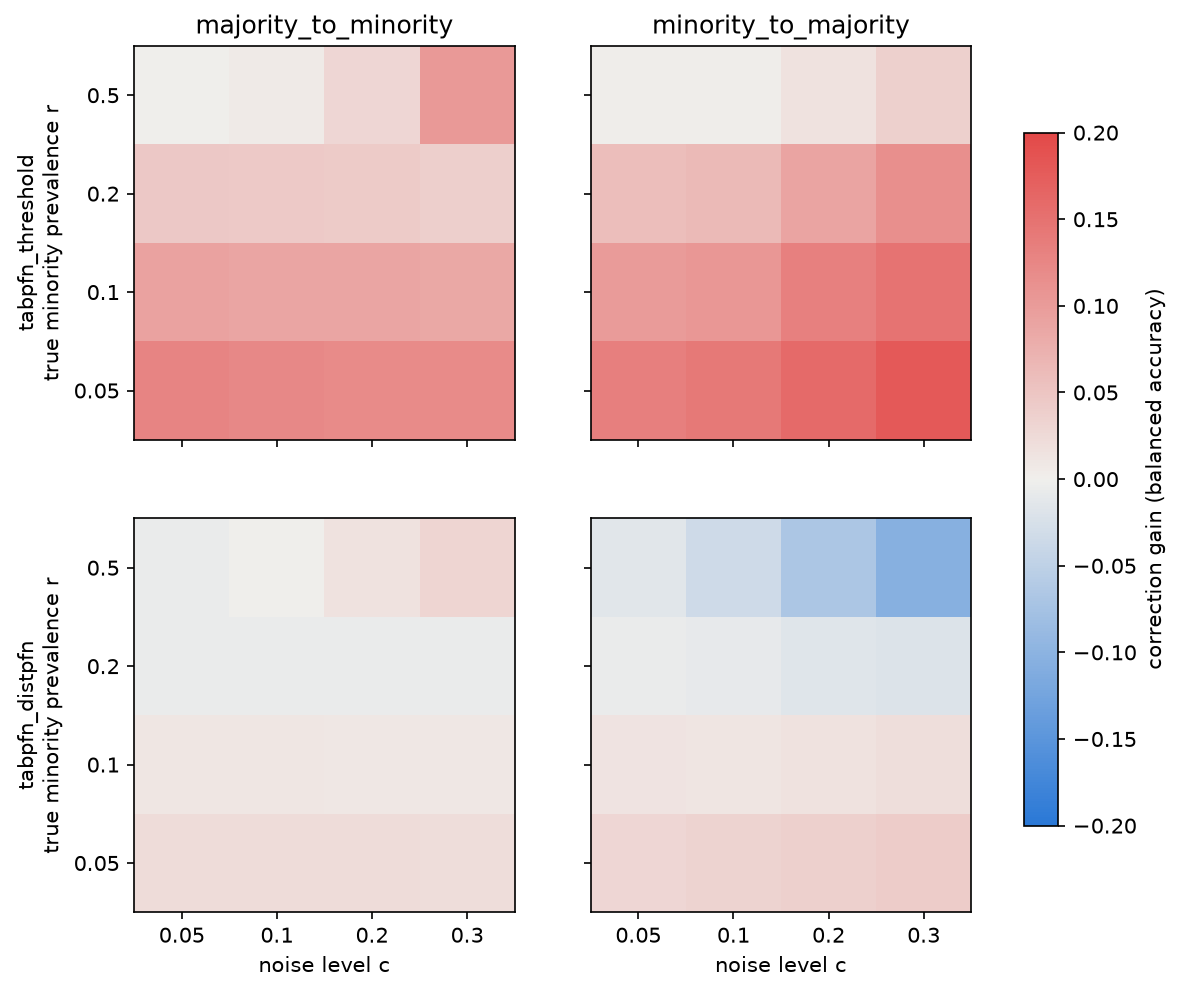
\includegraphics[width=0.85\linewidth]{figures/gain_heatmap_pair.png}
\caption{Correction gain (balanced accuracy) across $r$ and $c$ for
\texttt{tabpfn\_threshold} (top) and \texttt{tabpfn\_distpfn} (bottom), pooled
across 26 datasets and ten seeds. Blue marks cells where the correction hurt,
and red marks cells where it helped.}
\label{fig:gain-heatmap}
\end{figure*}

\subsection{Simplicity Outperforms Sophistication}
\label{sec:discussion-simplicity}

\texttt{tabpfn\_threshold} does less than any other correction. It shifts the
decision boundary from 0.5 to the class prior and nothing more
(Section~\ref{sec:methods-corrections}). It is nevertheless the most robust method
on discrimination (Table~\ref{tab:robustness}, Section~\ref{sec:results-rq1}),
with the lowest CHR and highest mean CG in both directions, and it leads on
break-even share too (Table~\ref{tab:breakeven}). Its calibration matches its
baseline by construction, since a threshold shift does not touch the predicted
probabilities (Section~\ref{sec:discussion-calibration} returns to why that is
not the same as leading on calibration). The two DistPFN variants sit at the
opposite end, with the highest CHR of any method in \emph{both} directions.

This builds on prior work. Elor and Averbuch-Elor~\cite{elor2022smote} found that
on clean data a well-tuned classifier often gains nothing from balancing and can
lose performance from it. This study shows that the same pattern holds, and
sharpens, once label noise is added. A correction can actively backfire, and in
this comparison the two most elaborate corrections backfire hardest on
discrimination while the simplest backfires least. Much of that backfiring is
concentrated at the balanced control $r{=}0.50$. Restricted to genuinely
imbalanced training sets ($r{\neq}0.50$), the DistPFN pair's Direction B CHR falls
from 43.8\%/47.4\% to 29.8\%/37.8\%, still four to twelve times
\texttt{tabpfn\_threshold}'s 0.3\% there (Section~\ref{sec:results-r050}). The
ranking does not change at any scope. A practitioner optimizing balanced accuracy
under uncertain label quality has, on these results, no clear reason to prefer a
more elaborate posterior-rescaling method over a threshold shift. That
recommendation does not cover every deployment, a point
Section~\ref{sec:discussion-calibration} returns to.

This may also reflect the study design. The severe-imbalance conditions combine
imbalance with a train/test prior mismatch, and threshold correction, DistPFN,
and DistPFN-T all target that mismatch. This may explain part of why
prior-adjusting corrections outperform resampling and cost-sensitive weighting in
general. It does not explain why the DistPFN variants fail more often than plain
threshold correction, which points to contamination robustness specifically.

\subsection{Robustness Check: Isolating the Balanced Control Condition ($r{=}0.50$)}
\label{sec:results-r050}

The headline numbers pool all four ratios, including $r{=}0.50$, a balanced
training set before contamination. To isolate it, every contribution metric and
statistical test is recomputed on $r \in \{0.20, 0.10, 0.05\}$ (hereafter
$r{\neq}0.50$) and on $r{=}0.50$ alone, using the same formulas and the same
already-collected evaluations. No model was retrained or re-scored.

Table~\ref{tab:robustness-r050} reports CHR and mean CG on $r{\neq}0.50$.
\texttt{tabpfn\_threshold} is unaffected in standing, and its Direction B CHR
falls from 2.4\% to 0.3\%. The DistPFN variants change substantially but not
completely. Under Direction B their pooled CHR of 43.8\%/47.4\% falls to 29.8\%
(\texttt{tabpfn\_distpfn}) and 37.8\% (\texttt{tabpfn\_distpfn\_t}) on
$r{\neq}0.50$, and their mean CG rises from $-0.004$/$-0.009$ pooled to
0.013/$-0.004$. At $r{=}0.50$ alone the same two methods fail 85.6\% and 76.0\% of
the time under Direction B, with mean gains of $-0.055$ and $-0.023$, and they
rarely reach break-even there (3.8\% of (dataset, $r{=}0.50$) pairs for both,
versus 46.2\%/47.4\% at $r{\neq}0.50$). Under Direction A the change is small. The
DistPFN pair's CHR moves from 35.1\%/33.9\% pooled to 34.9\%/35.9\%.
\texttt{tabpfn\_downsample}'s Direction A CHR does not fall when $r{=}0.50$ is
excluded (20.4\% pooled vs.\ 18.6\%), consistent with
Section~\ref{sec:discussion-direction}.

\begin{table}[t]
\centering
\caption{Correction Harm Rate and mean Correction Gain (balanced accuracy)
restricted to the imbalanced subset $r \in \{0.20, 0.10, 0.05\}$ ($n{=}312$ per
method and direction). Directly comparable to Table~\ref{tab:robustness}.}
\label{tab:robustness-r050}
\begin{tabular}{@{}lrrrr@{}}
\toprule
& \multicolumn{2}{c}{CHR} & \multicolumn{2}{c}{mean CG} \\
Method & Dir.\ A & Dir.\ B & Dir.\ A & Dir.\ B \\
\midrule
\texttt{xgb\_weighted}      & 0.115 & 0.032 & 0.028 & 0.043 \\
\texttt{xgb\_ros}           & 0.115 & 0.026 & 0.029 & 0.044 \\
\texttt{xgb\_smote}         & 0.106 & 0.029 & 0.026 & 0.041 \\
\texttt{tabpfn\_threshold}  & 0.032 & 0.003 & 0.084 & 0.119 \\
\texttt{tabpfn\_distpfn}    & 0.349 & 0.298 & 0.009 & 0.013 \\
\texttt{tabpfn\_distpfn\_t} & 0.359 & 0.378 & 0.004 & $-$0.004 \\
\texttt{tabpfn\_downsample} & 0.186 & 0.051 & 0.061 & 0.094 \\
\bottomrule
\end{tabular}
\end{table}

The Prior Sensitivity pattern changes too. At $r{=}0.50$, mean PSG for the DistPFN
pair under Direction A falls to $-0.058$/$-0.059$. On $r{\neq}0.50$ it turns
slightly positive ($+0.010$, $+0.009$), so the oracle prior modestly helps once
the balanced control is excluded. It remains negative under Direction B
($-0.013$, $-0.009$) and for \texttt{tabpfn\_threshold} in both directions
regardless of $r$. Every Friedman omnibus test remains significant on both the
$r{\neq}0.50$ and $r{=}0.50$-only subsets at both blocking levels ($p<10^{-8}$
throughout).

The core claims survive this check. No correction is uniformly safe, method
identity significantly affects balanced accuracy in every family and direction
with or without $r{=}0.50$, and \texttt{tabpfn\_threshold} remains the most robust
method, more clearly so once the balanced control is removed. What changes is the
size of the DistPFN pair's Direction B failure. A real share of it, though not
the majority, is a property of the balanced condition. Excluding $r{=}0.50$ cuts
the pair's Direction B CHR by roughly a third (43.8\%$\to$29.8\% and
47.4\%$\to$37.8\%), not down to the low single digits.

\subsection{Direction-Dependent Failure}
\label{sec:results-rq2}
\label{sec:discussion-direction}

Failure rates differ substantially between the two directed mechanisms, and the
direction of the difference depends on the method. Five of the seven methods have
a higher CHR under Direction A (majority rows relabeled as minority) than under
Direction B (minority rows relabeled as majority). These are \texttt{xgb\_ros},
\texttt{xgb\_smote}, \texttt{xgb\_weighted}, \texttt{tabpfn\_downsample}, and
\texttt{tabpfn\_threshold}, the last two by a wide margin
(Table~\ref{tab:robustness}). The two DistPFN variants show the opposite pattern.
Figure~\ref{fig:chr-regret} shows CHR and mean regret by method and direction.

This asymmetry is what class-conditional and asymmetric label-noise formalizations
predict~\cite{natarajan2013noisylabels,scott2013asymmetricnoise}, but it is large
enough to matter. A method's CHR under one direction is a poor predictor of its
CHR under the other. \texttt{tabpfn\_downsample}'s CHR is 20.4\% under Direction A
and 7.7\% under Direction B, nearly a threefold difference for the same method on
the same datasets. A robustness claim validated under one corruption mechanism, or
under symmetric random flips, does not transfer to a directed, class-conditional
error, and the true direction of label error is rarely known in advance. This is
the strongest argument in the study for testing every correction under both
directions.

\begin{figure*}[t]
\centering
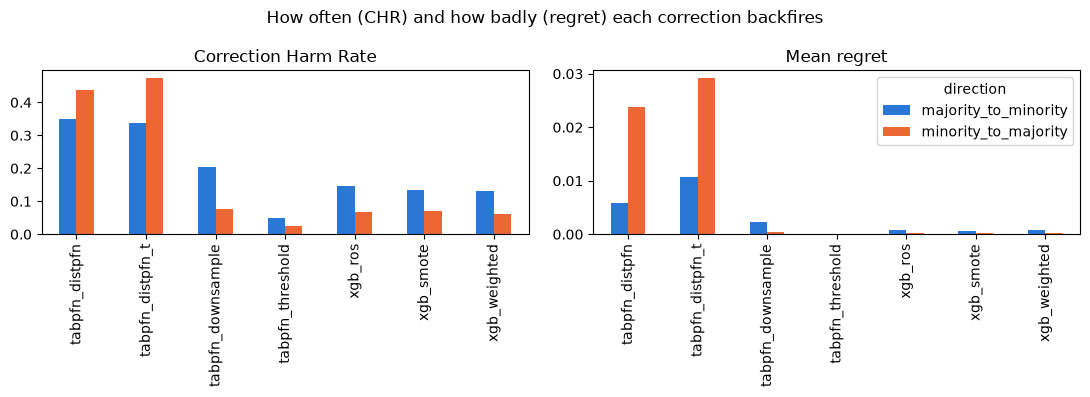
\includegraphics[width=0.85\linewidth]{figures/chr_regret.png}
\caption{Correction Harm Rate (left) and mean regret (right, $\max(0,-\text{CG})$)
by method and direction, over noisy blocks pooled across 26 datasets.}
\label{fig:chr-regret}
\end{figure*}

Regret and CHR tell a consistent story. The DistPFN pair has both the highest CHR
and the highest mean regret in both directions. Under Direction A,
\texttt{tabpfn\_distpfn\_t}'s mean regret (0.0108) is the highest of any method,
ahead of \texttt{tabpfn\_distpfn} (0.0059) and \texttt{tabpfn\_downsample}
(0.0023), even though \texttt{tabpfn\_downsample}'s CHR (20.4\%) sits below the
DistPFN pair's 33.9--35.1\%. Under Direction B the regret of
\texttt{tabpfn\_distpfn\_t} (0.0292) and \texttt{tabpfn\_distpfn} (0.0239) is an
order of magnitude above every other method, all of which are at 0.0004 or below.
\texttt{tabpfn\_threshold} has the lowest regret in both directions (0.0001 and
0.0000).

Part of this asymmetry traces to the uncorrected baselines. From $c{=}0$ to
$c{=}0.30$, balanced accuracy of \texttt{xgb\_none} falls by 0.076 (0.741 to 0.665)
under Direction B, against 0.034 (0.741 to 0.707) under Direction A, roughly 2.2
times as much. \texttt{tabpfn\_none} shows the same pattern, 0.066 against 0.032,
roughly 2.0 times. Losing genuine minority rows is more damaging to an uncorrected
model than diluting the minority class with mislabeled majority rows. This helps
explain why a correction's robustness under one direction does not predict its
robustness under the other.

\subsection{Break-Even Contamination Rates}
\label{sec:results-rq3}

Table~\ref{tab:breakeven} gives, for each method and direction, the share of the
104 (dataset, $r$) combinations (26 datasets $\times$ 4 ratios) whose
seed-averaged gain never drops to zero or below within the tested range, that is,
$c^*>0.30$. \texttt{tabpfn\_threshold} leads here too, staying net-beneficial
through the full range in 85.6\% of Direction A conditions and 87.5\% of Direction
B conditions. The lowest shares in both directions belong to the DistPFN pair,
40.4\% for \texttt{tabpfn\_distpfn} under Direction A and 32.7\% for
\texttt{tabpfn\_distpfn\_t} under Direction B. CHR counts every failing block
individually. Break-even share asks only whether a method's seed-averaged trend,
within one (dataset, $r$) combination, ever crosses zero. The two measures mostly,
but not perfectly, agree, which is why Section~\ref{sec:methods-contribution}
keeps CHR, Regret, and $c^*$ separate.

\begin{table}[t]
\centering
\caption{Share of (dataset, $r$) conditions, out of 104, where a method's
seed-averaged Correction Gain never dropped to zero or below within the tested
contamination range ($c^*>0.30$).}
\label{tab:breakeven}
\begin{tabular}{@{}lrr@{}}
\toprule
Method & Dir.\ A & Dir.\ B \\
\midrule
\texttt{xgb\_weighted}      & 69.2\% & 80.8\% \\
\texttt{xgb\_ros}           & 64.4\% & 80.8\% \\
\texttt{xgb\_smote}         & 62.5\% & 78.8\% \\
\texttt{tabpfn\_threshold}  & 85.6\% & 87.5\% \\
\texttt{tabpfn\_distpfn}    & 40.4\% & 37.5\% \\
\texttt{tabpfn\_distpfn\_t} & 41.3\% & 32.7\% \\
\texttt{tabpfn\_downsample} & 62.5\% & 74.0\% \\
\bottomrule
\end{tabular}
\end{table}

The corrupted prior explains less of a correction's failure than expected. On
average, the deployable observed-prior variant slightly outperforms the oracle
diagnostic rather than trailing it. Table~\ref{tab:psg} gives mean PSG
(Equation~\ref{eq:psg}) pooled and at $c{=}0.30$. Pooled, it is negative for all
three prior-dependent methods in both directions. The gap is not fixed, however.
At $c{=}0.30$ alone, \texttt{tabpfn\_threshold}'s mean PSG under Direction A is the
widest of the three, even though it is the most robust method on balanced
accuracy, so the ranking of prior sensitivity across methods is not stable.

\begin{table}[t]
\centering
\caption{Mean Prior Sensitivity Gap (Equation~\ref{eq:psg}), pooled across noisy
blocks and at $c{=}0.30$. Negative throughout: the oracle prior does not reliably
outperform the observed one.}
\label{tab:psg}
\begin{tabular}{@{}lrr@{}}
\toprule
Method / Direction & mean PSG (pooled) & mean PSG ($c{=}0.30$) \\
\midrule
\texttt{tabpfn\_threshold}, Dir.\ A  & $-0.012$ & $-0.037$ \\
\texttt{tabpfn\_threshold}, Dir.\ B  & $-0.008$ & $-0.019$ \\
\texttt{tabpfn\_distpfn}, Dir.\ A    & $-0.007$ & $-0.033$ \\
\texttt{tabpfn\_distpfn}, Dir.\ B    & $-0.020$ & $-0.043$ \\
\texttt{tabpfn\_distpfn\_t}, Dir.\ A & $-0.008$ & $-0.036$ \\
\texttt{tabpfn\_distpfn\_t}, Dir.\ B & $-0.014$ & $-0.033$ \\
\bottomrule
\end{tabular}
\end{table}

Figure~\ref{fig:psg} shows the observed and oracle curves. At low contamination they
stay close together. The two DistPFN variants separate sharply above $c{=}0.20$
under Direction A, with the oracle degrading faster, while
\texttt{tabpfn\_threshold} shows a comparable or larger separation at the highest
noise level. Even the true prior does not fully recover clean-condition performance
under severe contamination.

\begin{figure*}[t]
\centering
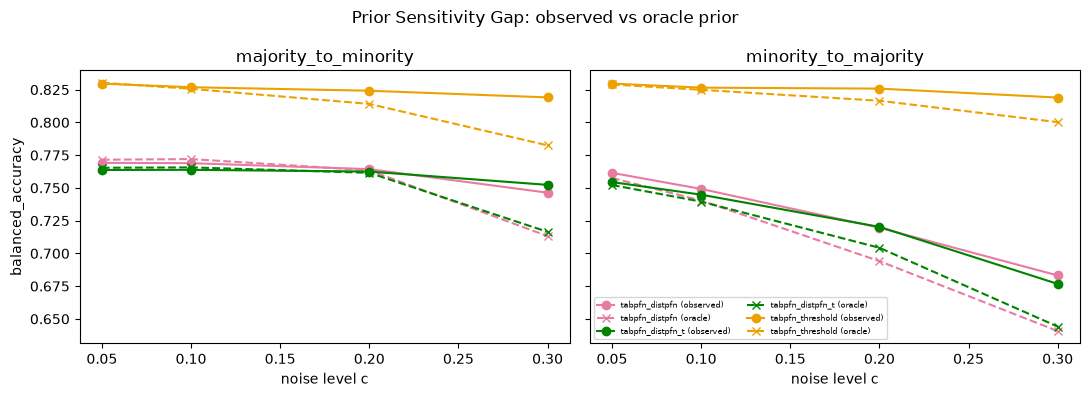
\includegraphics[width=0.85\linewidth]{figures/oracle_vs_observed.png}
\caption{Observed-prior (deployable, solid) versus oracle-prior (diagnostic,
dashed) balanced accuracy for the three prior-dependent TabPFN methods, pooled
across 26 datasets.}
\label{fig:psg}
\end{figure*}

\subsection{The Corrupted Prior Is Not the Main Failure Mode}
\label{sec:discussion-prior}

\label{sec:results-rq4}
The most surprising result is that mean PSG is negative for all three
prior-dependent methods in both directions. The true prior, which no deployment
could supply, does not reliably outperform the corrupted one. If the wrong prior
were the primary cause of these methods' decline, correcting it should have helped.
It does not, at least not under Direction B, or under Direction A at high
contamination. Restricted to $r{\neq}0.50$, mean PSG turns positive for both DistPFN
variants under Direction A ($+0.010$, $+0.009$). The corrupted prior therefore
contributes to their Direction A decline once the balanced control is excluded. It
is not the dominant effect that the more strongly negative figure at $r{=}0.50$
alone ($-0.058$/$-0.059$) suggests (Section~\ref{sec:results-r050}). The claim that
the corrupted prior is not the primary failure mode is strongest under Direction B,
increasingly so at high contamination for \texttt{tabpfn\_threshold}, and more
qualified for the DistPFN pair under Direction A at moderate contamination.

A structural reason follows from how these corrections work. All three adjust
TabPFN's output probabilities after the fact, using the class
prior~\cite{saerens2002adjusting,lee2026distpfn}. None of them touches the training
rows TabPFN reads as its in-context prompt~\cite{hollmann2023tabpfn,hollmann2025tabpfnv2}.
Contamination happens before any correction is applied, so the mislabeled rows stay
in that prompt whichever prior is supplied afterward. Swapping in the true prior
fixes the summary statistic the correction uses, but not the individual wrong
examples TabPFN has already been shown. This would explain why the oracle prior
helps so little. Confirming it would require an experiment this study did not run,
comparing a prior-only fix against a fix that also removes the mislabeled rows from
the context.

\subsection{Statistical Significance}
\label{sec:results-significance}

Table~\ref{tab:friedman} reports the Friedman omnibus test for each family and
direction, blocked by (dataset, $r$, $c$) ($n{=}416$). All four are significant at
$p<10^{-85}$, so method identity significantly affects balanced accuracy within both
families in both directions.

\begin{table}[t]
\centering
\caption{Friedman omnibus test statistics by family and direction. Condition
blocks are (dataset, $r$, $c$), $n{=}416$. Dataset blocks are one per dataset,
$n{=}26$, the more conservative check.}
\label{tab:friedman}
\label{tab:friedman-dataset}
\begin{tabular}{@{}llrrrr@{}}
\toprule
& & \multicolumn{2}{c}{Condition blocks} & \multicolumn{2}{c}{Dataset blocks} \\
Family & Direction & $\chi^2$ & $p$ & $\chi^2$ & $p$ \\
\midrule
XGBoost & Dir.\ A & 400.0 & $2.2\times10^{-86}$ & 46.8 & $3.7\times10^{-10}$ \\
XGBoost & Dir.\ B & 563.7 & $7.3\times10^{-122}$ & 47.4 & $2.9\times10^{-10}$ \\
TabPFN  & Dir.\ A & 681.7 & $3.1\times10^{-146}$ & 69.4 & $3.0\times10^{-14}$ \\
TabPFN  & Dir.\ B & 933.0 & $1.2\times10^{-200}$ & 71.5 & $1.1\times10^{-14}$ \\
\bottomrule
\end{tabular}
\end{table}

Blocking by (dataset, $r$, $c$) treats conditions from the same dataset as
independent evidence, although they share that dataset's feature distribution and
test set. The right-hand columns of Table~\ref{tab:friedman} repeat the comparison
with each dataset as a single block ($n{=}26$), the more conservative standard for comparing algorithms
across datasets (Section~\ref{sec:methods-statistics}). The $p$-values rise from
below $10^{-85}$ to between $10^{-14}$ and $10^{-9}$, but all four stay far below the
conventional $p<0.05$. Method identity affects balanced accuracy either way. The
(dataset, $r$, $c$) version overstates how strong that evidence is, not whether it
exists.

Pairwise tests (Holm-corrected) show where the differences lie. At the (dataset, $r$,
$c$) level, every uncorrected baseline differs significantly from every correction in
its family under Direction A. Under Direction B this holds for every XGBoost
correction and for \texttt{tabpfn\_threshold} and \texttt{tabpfn\_downsample}. Neither
DistPFN variant differs significantly from \texttt{tabpfn\_none} under Direction B
($p_{\text{Holm}}=0.58$ and $0.87$), despite their pooled CHR of 43.8\%/47.4\%. At the
dataset level, \texttt{tabpfn\_threshold} still differs significantly from every other
TabPFN method in both directions, so the finding that it is the most robust method
survives. The three XGBoost corrections become mutually indistinguishable in both
directions, though each still differs from \texttt{xgb\_none}. Under Direction B,
\texttt{tabpfn\_none}, \texttt{tabpfn\_distpfn}, and \texttt{tabpfn\_distpfn\_t} are
mutually indistinguishable ($p_{\text{Holm}}=1.00$ for all pairs). Under Direction A,
\texttt{tabpfn\_distpfn} is not significantly different from \texttt{tabpfn\_none}
($p_{\text{Holm}}=0.07$), and the two DistPFN variants are no longer distinguishable
from each other ($p_{\text{Holm}}=0.12$). None of the descriptive measures, CHR, mean
CG, or break-even share, depends on these tests. What changes is which differences a
formal test can support at $n{=}26$. The DistPFN pair's Direction B failure is real
and large by descriptive measures, but not statistically distinguishable from the
null at the dataset-level standard.

\subsection{Calibration Reliability and Accuracy}
\label{sec:results-reliability}
\label{sec:discussion-calibration}

Figure~\ref{fig:reliability} tracks Brier score and expected calibration error (ECE)
against noise level. Every XGBoost correction improves on \texttt{xgb\_none} at every
noise level tested, in both directions. \texttt{tabpfn\_downsample} is worse-calibrated
than the uncorrected \texttt{tabpfn\_none} on both ECE and Brier score at every noise
level under Direction A, the only method in the study with that pattern on either
metric. \texttt{tabpfn\_threshold} never exceeds its baseline's Brier score or ECE in
either direction. This follows from how it works. It moves only the decision threshold,
so the probabilities that Brier score and ECE measure are identical to those of
\texttt{tabpfn\_none} by construction. \texttt{tabpfn\_distpfn} and
\texttt{tabpfn\_distpfn\_t} are the two best-calibrated methods of any tested, correction
or baseline, at every noise level in both directions. They also have the highest CHR on
balanced accuracy (Section~\ref{sec:results-rq1}). Discrimination and calibration are
therefore different failure modes. A correction that often underperforms its baseline on
discrimination can still assign well-calibrated probabilities.

\begin{figure*}[t]
\centering
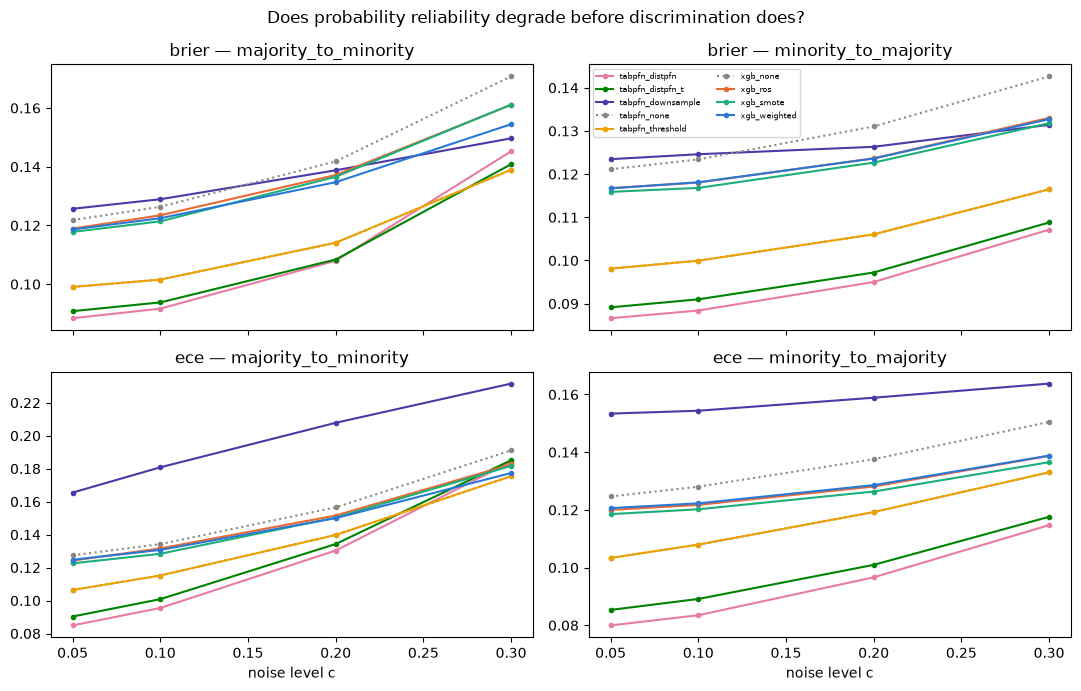
\includegraphics[width=0.85\linewidth]{figures/reliability.png}
\caption{Brier score (top) and expected calibration error (bottom) against noise level,
faceted by direction, pooled across 26 datasets. Dotted gray lines mark the two
uncorrected baselines.}
\label{fig:reliability}
\end{figure*}

Balanced accuracy and calibration measure different properties, and a correction can
excel at one while failing at the other. That matters for deployment. A system that
only needs a correct label cares mainly about discrimination, and by that standard the
DistPFN variants are a poor choice under contamination. A system that acts on predicted
probabilities, for example by setting a risk threshold, allocating a limited budget, or
ranking cases by urgency, cares about calibration first. For that use, the pair's CHR is
the wrong reason to rule them out. Reporting CHR and mean CG alone would also miss that
\texttt{tabpfn\_downsample} is uniquely poor on calibration under Direction A, even though
its balanced accuracy profile looks far more favorable there, with the second-highest
mean CG of any method. Deployment requires checking both axes separately rather than
inferring one from the other.

\subsection{Implications for Imbalance Correction Under Label Noise}
\label{sec:discussion-implications}

Related work on imbalance and label noise as a joint problem has proposed new
training-time algorithms: combining cleaning with resampling~\cite{koziarski2020ccr},
active learning with noisy-label training~\cite{khanal2024activelabel}, class-balanced
sample selection~\cite{liu2024imbalancednoisy}, or deliberately engineered label noise
that corrects a known class bias~\cite{hu2025beneficialnoise}. This study asks a
different question: whether the corrections practitioners already use need replacing at
all. The answer depends on which correction is in use. \texttt{tabpfn\_threshold} stays
net-beneficial through the full contamination range in 85.6\% to 87.5\% of conditions
(Table~\ref{tab:breakeven}), the highest share in both directions, so switching to it may
fix most of what a new algorithm would need to solve. The DistPFN variants fail badly on
discrimination under high contamination in both directions on the full pool, so for a
deployment that needs a correct label the case for joint noise-and-imbalance-aware
training remains strong. How this choice depends on the deployment's needs is set out in
Section~\ref{sec:discussion-calibration}. Telling these situations apart requires an
audit of this kind, not a default assumption that a published correction is safe or
unsafe on every axis a deployment cares about.

\section{Threats to Validity}
\label{sec:threats}

\subsection{Internal Validity}
\label{sec:threats-internal}

Every \texttt{tabpfn\_*} result in this paper comes from one checkpoint,
verified by SHA-256 hash (Section~\ref{sec:methods-implementation}),
and uses Apple's Metal GPU backend for inference. The whole study,
XGBoost included, ran on one machine
with every library forced to a single thread to avoid a documented
XGBoost/PyTorch conflict. A different checkpoint, backend, or thread
count could shift specific numbers, but there is no reason to expect
the broader pattern, that robustness varies by method and direction,
to depend on any of them. Each (dataset, ratio, contamination rate,
direction) combination was repeated across ten seeds to reduce
dependence on a single train/test split or
corruption realization. Ten repetitions still provide only limited
precision for quantities determined by whether a
seed-averaged value crosses zero, including Correction Harm Rate and
the break-even rate. Additional seeds would further improve
uncertainty characterization of both measures, a limitation
Section~\ref{sec:threats-construct}'s break-even non-monotonicity
finding may partly reflect.

The claim that robustness varies by direction carries its own caveat.
Direction A's and Direction B's contamination rate $c$ are defined against
different reference points (Section~\ref{sec:methods-corruption}), so a
matched nominal $c$ does not correspond to a matched absolute flip count
between the two. Direction A flips a larger fraction of $n_{\min}$'s worth
of rows than Direction B at every tested $c$ above zero. The finding that
direction changes how often a correction fails should be read as a
comparison between two distinct, realistically motivated corruption
processes at their own natural severity levels, not as a
magnitude-controlled manipulation of direction alone. A shared flip-count
definition was considered and rejected, since the two most natural
candidates either require flipping more minority rows than exist at
$r{=}0.05$, or introduce an $r$-dependent mismatch between directions
that grows increasingly severe as $r$ decreases. That mismatch would be
worst precisely at the most imbalanced settings this study emphasizes,
worse than the fixed, $r$-independent gap the current design carries at
every tested $r$.

A related caveat applies to the imbalance ratio $r$ itself. The test
partition is never resampled and keeps each dataset's natural class
distribution (Section~\ref{sec:methods-datasets}), while training is
deliberately pushed to $r$, so the low-$r$ conditions this study
emphasizes combine imbalance with train and test prior shift rather than
isolating imbalance alone. This is the standard evaluation paradigm
across the class-imbalance literature. Training on a rebalanced set and
testing on the natural population is what makes a correction's benefit
deployment-relevant in the first place, but it means this study cannot
cleanly attribute a method's robustness to tolerance of imbalance
specifically as opposed to tolerance of prior shift. This matters most
for \texttt{tabpfn\_threshold}, \texttt{tabpfn\_distpfn}, and
\texttt{tabpfn\_distpfn\_t}, whose underlying mechanism directly targets
prior mismatch (Section~\ref{sec:discussion-simplicity}). A design that
resampled the test partition to match each tested $r$ would remove this
coupling, at the cost of evaluating performance on a population that
does not correspond to any dataset's actual distribution. Consequently,
the present results should be read as robustness under the joint
imbalance/prior-shift setting that rebalanced training and
natural-distribution testing together induce, not as a causal estimate
of imbalance tolerance in isolation.
Section~\ref{sec:results-r050} partially addresses a related but distinct
concern, whether the balanced ratio $r{=}0.50$ (not imbalanced even
before contamination) was itself driving the pooled headline numbers, by
recomputing every contribution metric and statistical test with
$r{=}0.50$ isolated from $r \in \{0.20, 0.10, 0.05\}$. The results
confirm that a substantial share of the DistPFN pair's apparent harm
under Direction B is concentrated at that one ratio. This does not
resolve the train/test prior-shift coupling described above, which
remains present within the $r{\neq}0.50$ subset itself, but it does rule
out $r{=}0.50$ specifically as an unexamined confound in the headline
comparisons.

One correction method's construction interacts with a subset of datasets
in a way worth naming directly. \texttt{xgb\_smote} synthesizes new
minority rows by interpolating in the feature space actually presented to
it, the already-imputed, one-hot-encoded representation
(Section~\ref{sec:methods-datasets}), not the raw categorical values. For
the seven datasets with genuinely categorical columns, this means a
synthetic row can carry a fractional value for what should be a one-hot
indicator, e.g.\ 0.37 rather than 0 or 1, mathematically usable by
XGBoost's tree splits but not a valid category membership.
\texttt{xgb\_ros} is unaffected, since it duplicates real rows rather than
interpolating between them. This is standard practice for applying
off-the-shelf SMOTE to mixed-type data, not an implementation error
specific to this study, and auditing correction methods as they are
commonly deployed, rather than in a bespoke mixed-type-aware variant, is
consistent with this study's stated aim
(Section~\ref{sec:methods-corrections}). Restricting \texttt{xgb\_smote}'s
headline numbers to the 19 datasets with no categorical columns changes
them only slightly: CHR moves from 13.5\%/7.2\% (pooled,
Table~\ref{tab:robustness}) to 13.5\%/6.2\%, and mean CG from
0.023/0.033 to 0.026/0.037, so the categorical datasets are not driving
this method's measured robustness.

\subsection{External Validity}
\label{sec:threats-external}

The 26 datasets audited range from 270 to 60{,}000 raw rows
(Table~\ref{tab:datasets}), but the raw row count is not what any method
actually fits on. The controlled training set every stress cell draws
from is capped by $N_{\text{common}}$ (Section~\ref{sec:methods-ncommon}),
which tops out at 18{,}698 rows even for Adult, the dataset with the
largest minority class in raw terms, because minority availability at
$r{=}0.50$ is the binding constraint regardless of how many majority rows
the raw dataset has. Every condition
tested therefore stays well within TabPFN's intended small-tabular-data
regime but far from the scale where gradient-boosted methods are
typically deployed. Whether the same robustness ranking holds on larger,
higher-dimensional, or more categorical-heavy tabular data, or simply on
a dataset whose minority class alone is large enough to push
$N_{\text{common}}$ higher, is untested. Every dataset audited is also a
binary-classification problem. Whether the same corrections and the same
robustness patterns extend to multi-class imbalance, where a correction
may need to reweight several minority classes at once rather than one, is
untested as well.

The two corruption mechanisms audited are both
class-conditional (Section~\ref{sec:methods-corruption}). The flip
probability depends only on the true class, not on the specific
feature values of the row being flipped. Real-world label noise is
often instance-dependent instead, arising from cases that are
genuinely ambiguous or that share features with the other class, and
this study says nothing about whether the same methods stay robust
under that kind of noise. The four tested contamination rates also stop
at 0.30, with results never extrapolated beyond that point
(Section~\ref{sec:methods-contribution}), so this study cannot say
whether the same patterns hold at higher contamination. Each stress cell
also applies exactly one corruption direction at a time, never a mixture
of both within the same corrupted training set. Real-world label noise
plausibly combines both directions at once, and this study does not test
whether a correction's robustness under one direction in isolation
predicts its robustness once both are present together.

\subsection{Construct Validity}
\label{sec:threats-construct}

Correction Gain, Correction Harm Rate, Regret, and the break-even rate
are original to this paper. They are reported here only on balanced
accuracy, not on the other nine metrics tracked in
Section~\ref{sec:methods-metrics}. A correction ranked robust by CHR
on balanced accuracy is not guaranteed to be equally robust by the
same measure on AUPRC or minority recall, a point the calibration
results in Section~\ref{sec:results-reliability} already illustrate
for a different metric pair. The break-even rate itself assumes a
correction's gain declines monotonically as contamination rises, an
assumption this study's own data does not fully support. Of the 522
(method, dataset, ratio, direction) combinations with a defined
break-even point, 54.6\% show the seed-averaged gain recover to
positive at a higher contamination level after already crossing zero
at a lower one, a majority, not a minority, of defined break-even
points. $c^*$ marks the first noise level a correction stops
paying off, not a guarantee that it stays that way at every higher
level tested. The Prior Sensitivity Gap's oracle
variant assumes access to the true, pre-corruption class prior,
something no real deployment has. It is a diagnostic construct, not a
claim about achievable performance, and Section~\ref{sec:results-rq4}
found it is not even reliably better than the observed-prior variant
it is meant to bound.


\section{Conclusion and Future Work}
\label{sec:conclusion}

This paper set out to test whether standard imbalance corrections
remain worth applying once the labels they depend on cannot be
trusted. Across 26 datasets, seven correction methods spanning two
model families, and two directed label-error mechanisms, every
correction audited underperformed its matched uncorrected baseline in
at least some tested condition. How often and how badly it did so
depended on the method, on the direction of the label error, and on
whether balanced accuracy or calibration was the metric being judged,
never on a single number alone.
The simplest correction tested, a threshold shift keyed to the class
prior, was consistently the most robust on discrimination, leading
every other method on Correction Harm Rate and mean Correction Gain in
both directions. The two most mathematically involved corrections,
DistPFN and DistPFN-T, held the highest Correction Harm Rate of any
method under both directions, more than five times the next-highest
method's rate under Direction B, the opposite of what their added
sophistication might suggest, yet those same two corrections were also
the best-calibrated methods in the entire study. A robustness check
restricted to genuinely imbalanced training sets, excluding the
balanced $r{=}0.50$ control, shows a real share, though not the
majority, of that harm rate concentrated at the balanced condition
specifically: the DistPFN pair's Direction B Correction Harm Rate
falls from 43.8\%/47.4\% to 29.8\%/37.8\% once $r{=}0.50$ is excluded,
while \texttt{tabpfn\_threshold}'s lead over the rest of the field
holds or strengthens throughout. A correction that more frequently
degrades discrimination relative to its uncorrected baseline can
nevertheless produce better-calibrated probabilities, a split this
paper's results surface rather than resolve in either method's favor.

The five contribution metrics introduced here, Correction Gain,
Correction Harm Rate, Regret, the break-even contamination rate, and
the Prior Sensitivity Gap, made this possible, separating whether a
correction helps from how often it fails, how badly it fails when it
does, and how much of that failure traces to the corrupted prior
specifically. The same framework also
surfaced a result this paper did not anticipate, that the corrupted
prior is not the primary reason TabPFN's posterior-rescaling
corrections decline under contamination, since handing them the true
prior did not reliably help, and on average even hurt slightly.
Section~\ref{sec:discussion-prior} offers one explanation, that these
corrections never touch the mislabeled rows still sitting in TabPFN's
in-context prompt.

Several directions follow from what this study leaves open. Confirming
the explanation above would need an experiment that cleans the
mislabeled rows from TabPFN's in-context prompt directly, rather than
only adjusting the prior applied to it; separately, because training
here is deliberately pushed to each tested ratio while the test
partition keeps each dataset's natural class distribution, a complementary
matched-prior evaluation regime, resampling the test partition to match
each tested $r$ rather than keeping it at the dataset's natural
prevalence, would isolate how much of a prior-adjusting method's
robustness, particularly \texttt{tabpfn\_threshold}'s, reflects imbalance
tolerance specifically rather than the train/test prior mismatch the
present design creates; it targets a different, less deployment-oriented
question than the one this study poses, so it belongs alongside these
results as a complementary direction rather than as an outstanding gap in
them. Beyond those two, testing whether
the same robustness ranking holds on a dataset whose minority class
alone permits a larger controlled training set, on tabular foundation
models other than TabPFN, under multi-class imbalance, and under
instance-dependent or simultaneous-direction label noise rather than
the class-conditional, single-direction mechanisms audited here, are
the most direct ways to extend this audit.

\bibliographystyle{ACM-Reference-Format}
\bibliography{references}

\end{document}
